\documentclass[a4paper,11pt]{article}
\usepackage[margin=2cm]{geometry}

\usepackage[nodayofweek]{datetime}
\longdate
\usepackage{algorithm}
\usepackage{algpseudocode}
\usepackage{graphicx}
\usepackage{enumitem}
\usepackage{fancyhdr}
\usepackage{float}
\usepackage{array}
\usepackage{multirow}
\usepackage{amsmath}
\usepackage{textcomp}
\usepackage{tabularx,ragged2e,booktabs,caption}
\usepackage{hyperref}
\usepackage{url}
\usepackage{fancyhdr}
\usepackage{subcaption}

\usepackage[utf8]{inputenc}
\usepackage{pdfpages}
\captionsetup{skip=0pt}
\newcolumntype{P}[1]{>{\centering\arraybackslash}p{#1}}
\newcolumntype{M}[1]{>{\centering\arraybackslash}m{#1}}
\pagestyle{fancyplain}
\fancyhf{}
\lhead{\fancyplain{}{M.Sc.\ Group Project Report}}
\rhead{\fancyplain{}{\today}}
\cfoot{\fancyplain{}{\thepage}}


\title{Online-Learning in Social Networks\\\Large{--- Report Two ---}}
\author{Shanshan Fu, Oh Boon Eng, Ani Petrosyan, Magdalena Sadowska,
  Shahrokh Shahi, Yunxin Zhou\\
       \{sf2715,beo12,ap7614,ms915,ss6515,yz5115\}@ic.ac.uk\\ \\
       \small{Supervisor: Dr.\ Alessandra Russo}\\
       \small{Course: CO530/533, Imperial College London}
}

\begin{document}
\maketitle

\tableofcontents
\newpage
\setcounter{page}{1}
\section {Introduction}

Today, with around 3 billion people using some form of the Online Social Network (OSN)\cite{InternetUsers}, the difficult challenge of preserving one\textquotesingle s privacy whilst still fulfilling their social needs is almost inevitable. In order to decrease such difficulty, OSN platforms often allow the uploaders to define a target audience of the information they post. However, some of the members of the preselected group may choose to re-share the information, which could lead to unexpected privacy breaches\cite{PrivacyBreaches}. As a result, the uploaders might not always anticipate the negative consequences of their online activities and engage in actions that they may later regret\cite{FacebookRegret, ShareRegret}.\\
\indent The aim of this project is to develop a web plugin based on the research conducted by Imperial College London. The study proposes a Learning to Share product, in which a parametric Markov chain (PMC), a chain with unknown transition probabilities, is utilised to evaluate the privacy risk and social benefit of sharing an information with each friend or a member of a predefined target audience. The main functionality of the web plugin is to be able to identify potential malicious friends based on previous interactions between the user and his/her friends and return an appropriate warning message to the user when the user wants to share a post with said friends so as to prevent the user from sharing information that may be leaked to unintended audiences.\\
\indent The approach models the interactions  between  the  user  and  each  group  member  as a discrete-time Markov chain (DTMC) with parameterised transition probabilities.  These probabilities are learnt and continually updated at run-time, based on the actual interactions between the user and the group member.  Whenever the user considers sharing a new message with a group member, the parametric DTMC is formally verified to establish whether the member still meets the user's sharing requirements. These requirements specify the maximum level of privacy risk and the minimum level of social benefit that he user is willing to accept in order to share the new message with the group member. The requirements take into account the sensitivity level of the message, and are formally expressed in probabilistic temporal logic.\\
\indent Being currently the most widely used OSN that provides a variety of user interactions\cite{RankSN, Interactions}, Facebook will be considered as the prominent case study in this project.\\
 
 \subsection{Background}
 
 \subsection{Learning to Share Approach}

 
 
\subsection{Facebook Terminology}


Facebook has many features. Within this project, those components that are common in most of the social networks are of interests. To establish a tool relating the user’s privacy, acquaintance with these features is inevitable. The crucial components of Facebook are as follows:
\\\\
\noindent \textbf{Timeline:} The Timeline can be considered as the main feature of the Facebook in which all the contents of the user’s profile, including posts, photos, videos, etc., are categorized and depicted according to the period of time in which they are posted or created. The Timeline is actually a new version of the Wall that was the regular space of the user’s content.
\\\\
\noindent \textbf{Like:}
Like is a way to give positive feedback to contents, e.g. posts, comments, photos, etc. Recently, Facebook launched its new "reaction" buttons, giving users the option of using "reactions" such as "Love" "haha" "Wow" "Sad" and "Angry" in stead of Like.
\\\\
\noindent \textbf{Notifications:}
Notifications tell the user that something has been updated in his or her profile page or in a friend’s status, if he or she has been specified as a close friend. These updates can be a comment on a picture of the user, an answer to a user’s comment, a message posted on user’s timeline, etc. The user will be notified by a notification counter in red at the top of the page, which if clicked displays the most recent ones.
\\\\
\noindent \textbf{Friends:}
The fundamental functionality of a social network is friending that is adding someone to a list of “friends” who the user wants to have interaction with. The act of friending someone grants the privilege of viewing and posting on the user’s timeline. 
\\\\
\noindent \textbf{News Feed:}
This component enables user’s to track of the others’ activities, such as new posts, photos, life events.

\subsection {Report Structure}
\indent This report describes the development process of the plugin. It is divided into the following sections:

\begin{itemize}

\item \textbf{Specification:} The requirements of the each component of the plugin, broken down into small tasks for the members of the group to handle.

\item \textbf{Design:} Detailed description of the web plugin and the functionalities of each of its components.

\item \textbf{Methodology:} Development technique adopted by the group, issues faced during the development process as well as testing methodology.

\item \textbf{Group Work:} Assignment of tasks to each group member

\item \textbf{Final Product:} 

\end{itemize}

\section{Specification}

ADD SOME STUFF HHERE
\subsection{Requirements}
\noindent Main high level essential requirements of the web plugin proposed by the research group include the creation of a component, that is responsible for monitoring the social interaction between the user and each friend, a user interface that allows the user to specify his/her settings, as well as adding an automatic manager responsible for recommendation to the user to select a proper audience group. Table 1 demonstrates the low level specifications derived from the aforementioned requirements by applying the simplified version of van Lamsweerde\textquotesingle s KAOS goal-oriented model \cite{KAOS}, questioning how and why a particular requirement is applied. Table 1 is grouped by a particular component of the plugin and includes a relevant risk levels.

 \begin{table}[H]
\small
\captionof{table}{Specifications} \label{tab:title2} 
 \begin{tabular}{|c|M{4cm}|m{9.5cm}|c|}
 \hline
 & \textbf{Component} & \textbf{Description of Specifications} & \textbf{Risk*}\\
 \hline
 \parbox[t]{2mm}{\multirow{25}{*}{\rotatebox[origin=c]{90}{Minimum Specifications}}} &
\multirow{4}{*}{Facebook API} & Creating an interface to get permission from user through facebook API&L\\[1ex]
\cline{3-4}
&&
Creating a user interface that allows the user to input the level of sensitivity as well as the privacy risk and social benefit thresholds &L\\[3ex]
 \cline{2-4}
& Database &
Creating a database in form of a hash table to store information and sensitivity level&L\\[2ex]
\cline{2-4}
& Monitor Module & Keeping track of interactions between the user and selected friends &H\\
 \cline{2-4}
& Parametric Model Checker &
Integrating of existing parametric Markov chain model with the application&L\\[2ex]
 \cline{2-4}
& Online Parameter Learning Engine &
Integrating of existing code that updates the parameters of the parametric Markov chain model &L\\[3ex]
 \cline{2-4}
& \multirow{6}{*}{\begin{minipage}{4cm}\center{Adaptive Sharing Analyzer}\end{minipage}} & Creating a privacy risk and social benefit calculator &L\\[2ex]
\cline{3-4}
&&Verifing if the user specified sharing preferences are met &L\\[1ex]
\cline{3-4}
&&Calculating utility trade-off between social benefit and privacy risk&H\\[1ex]
\cline{3-4}
&&Identifying the potential malicious friends and report them to the user&L\\[1ex]
\hline
\parbox[t]{2mm}{\multirow{10}{*}{\rotatebox[origin=c]{90}{Possible Extensions}}} & Database &
Development of a database in place of hash table storing relevant data&L\\[2ex]
 \cline{2-4}
& Online Learning Model &
Automate the generation of the online learning model for any online social network based on the activity diagram on the network&H\\[3ex]
 \cline{2-4}
& Level of Sensitivity &
Explore machine learning methods and algorithms to improve determination of level of sensitivity&H\\[2ex]
 \cline{2-4}
& Parametric Model Checker &
Automate  producing the algebraic expression through PRISM for other social networks&H\\[2ex]
 \cline{2-4}
& Plugin Support&
Extension of the plugin to support multiple browsers and exploring the possibility of support on mobile devices&H\\[2ex]
\hline
 \end{tabular}
*Risk index is categorised as high (H) or low(R), depending on its impact and occurrence. The following were considered in the classification: human, i.e. lack of development experience, software, being bugs with chosen tools and frameworks, and schedule, meaning inability to complete given specifications within given time framework.
 \end{table}
\indent Additionally, the non-functional specifications that need to be taken into consideration are performance and security. As far as performance is concerned, the application of concurrency will be implemented. The security, on the other hand, will be met by a strict implementation of Facebook API, as well as a thorough testing of the plugin. 
\\
\indent Initially, the essential requirements of the web plugin were concerned with monitoring social interactions within a user\textquotesingle s post in a group. However, after application of the said KAOS goal model, it became obvious that monitoring of the user\textquotesingle s post in a group would not be feasible. More specifically, during the research concerning how to implement such an aspect, it was discovered that selecting the target audience of shared information is not allowed, therefore making it impossible for the web plugin to enable the exclusion of malicious members. That discovery led to a significant change in requirements from the group setting to monitoring of the Facebook Timeline activities, which introduced a new probabilistic model, as described in Section 2.

\subsection{Updates to the original specification}

The Table 1 summarises the progress of the project to date.

 \begin{table}[H]
\captionof{table}{Minimum requirements} \label{tab:title2} 
\hspace*{-0.1in}
 \begin{tabular}{|M{3.2cm}|m{9.7cm}|c|c|}
 \hline
 \textbf{Component} & \textbf{\space \space \space \space \space \space \space \space \space \space \space \space \space \space \space \space \space \space \space \space \space \space \space \space \space \space \space \space \space Tasks} & \textbf{ECD*} &  \textbf{Status}\\
 \hline
 \multirow{4}{*}{User Input Plugin} &
Creating a log-in section&Phase 1&Completed\\
\cline{2-4}
&Getting access token from Facebook&Phase 1&Completed\\
\cline{2-4}
&Creating settings section&Phase 1&Completed\\
\cline{2-4}
&Creating warning message section&Phase 1&Completed\\
\cline{2-4}
&Creating server to pass and obtain information between plugin and monitor&Phase 1&In progess\\
 \hline
\multirow{5}{*}{Monitor Module} &Getting user\textquotesingle s friends list&Phase 1&Completed\\
\cline{2-4}
&Accessing user\textquotesingle s notifications to track the interactions&Phase 1&Completed\\
\cline{2-4}
&Fetching all of the user\textquotesingle s posts, related comments and likes&Phase 1&Completed\\
\cline{2-4}
&Calculating the transition probabilities for Parametric Model Checker&Phase 1&Completed\\
\cline{2-4}
&Integrating the monitor with the other parts&Phase 1&Completed\\
\hline
Parametric Model Checker &
Refactoring the code to work with the real time data&Phase 1&Completed\\
\cline{2-4}
&Integrating the code with the plug-in&Phase 1&Held up\\
\hline
Online Parameter Learning Engine &
Integration of existing code that updates the parameters of the parametric Markov chain model&Phase 1&In progess\\
\hline
\multirow{5}{*}{Adaptive Sharing} & Privacy risk calculator&Phase 1&Completed\\
\cline{2-4}
&Social benefit calculator &Phase 1&Completed\\
\cline{2-4}
&Utility trade-off calculator&Phase 1&Completed\\
\cline{2-4}
Analyser&Creating a method to compare the outcomes with user specified preference &Phase 1&Held up\\
\hline
 \end{tabular}
\small{*ECD - Expected Completion Date}
 \end{table}

Although significant progress with regard to the development of the plugin has been made, two essential requirements were marked as held up. Also, the current stage of the plugin development can be evaluated to Phase Two as opposed to initially estimated Phase Three. The reasoning behind the delay is a number of limitations encountered during the development, as presented in the following sections (2.1 and 2.2).

\subsection {Specifications Update}

The table below provides the updates to the specifications described in Table 1.
 \begin{table}[H]
\captionof{table}{Updated Specifications} \label{tab:title2}
\hspace*{-0.3in}
 \begin{tabular}{|M{4.5cm}|m{11.5cm}|c|}
 \hline
\textbf{Component} & \textbf{\space \space \space \space \space \space \space \space \space \space \space \space \space \space \space \space \space \space \space \space \space \space \space \space \space \space \space \space Description} & \textbf{ECD}\\

 \hline
User Login &
Submitting a review to Facebook to obtain required permissions & Phase 2\\

\hline
\multirow{4}{*}{User Input Plugin} &
Developing messaging system to communicate between two types of plugins & Phase 2 \\

\cline{2-3}
&Researching whether accessing Facebook’s DOM is a practically feasible solution & Phase 2\\

\cline{2-3}
&Adding terms and conditions and user agreement page & Phase 2\\

\cline{2-3}
&Exploring an alternative construction of the plugin consisting of only one type, i.e. the popup & Phase 2\\

\hline
Monitor Module & Coming up with a reliable way to read the user's notifications, making sure none of the interations are missed & Phase 2\\

\hline
Parametric Model Checker &
Updating the model to include Facebook's new feature (reactions) & Phase 2\\

\hline
 \end{tabular}
 \end{table}

\subsection {Schedule updates}
The major update to the schedule includes extension of the Phase One from 13th to 27th of March due to reasons listed in Section 2.1 and 2.2. The final deadline applies to all of the components, as each  is being developed concurrently by each member of the team. Moreover, due to extension of the Phase One, the remaining Phases had to be shortened.

\begin{figure}[H]
	\hspace*{-0.26in}
	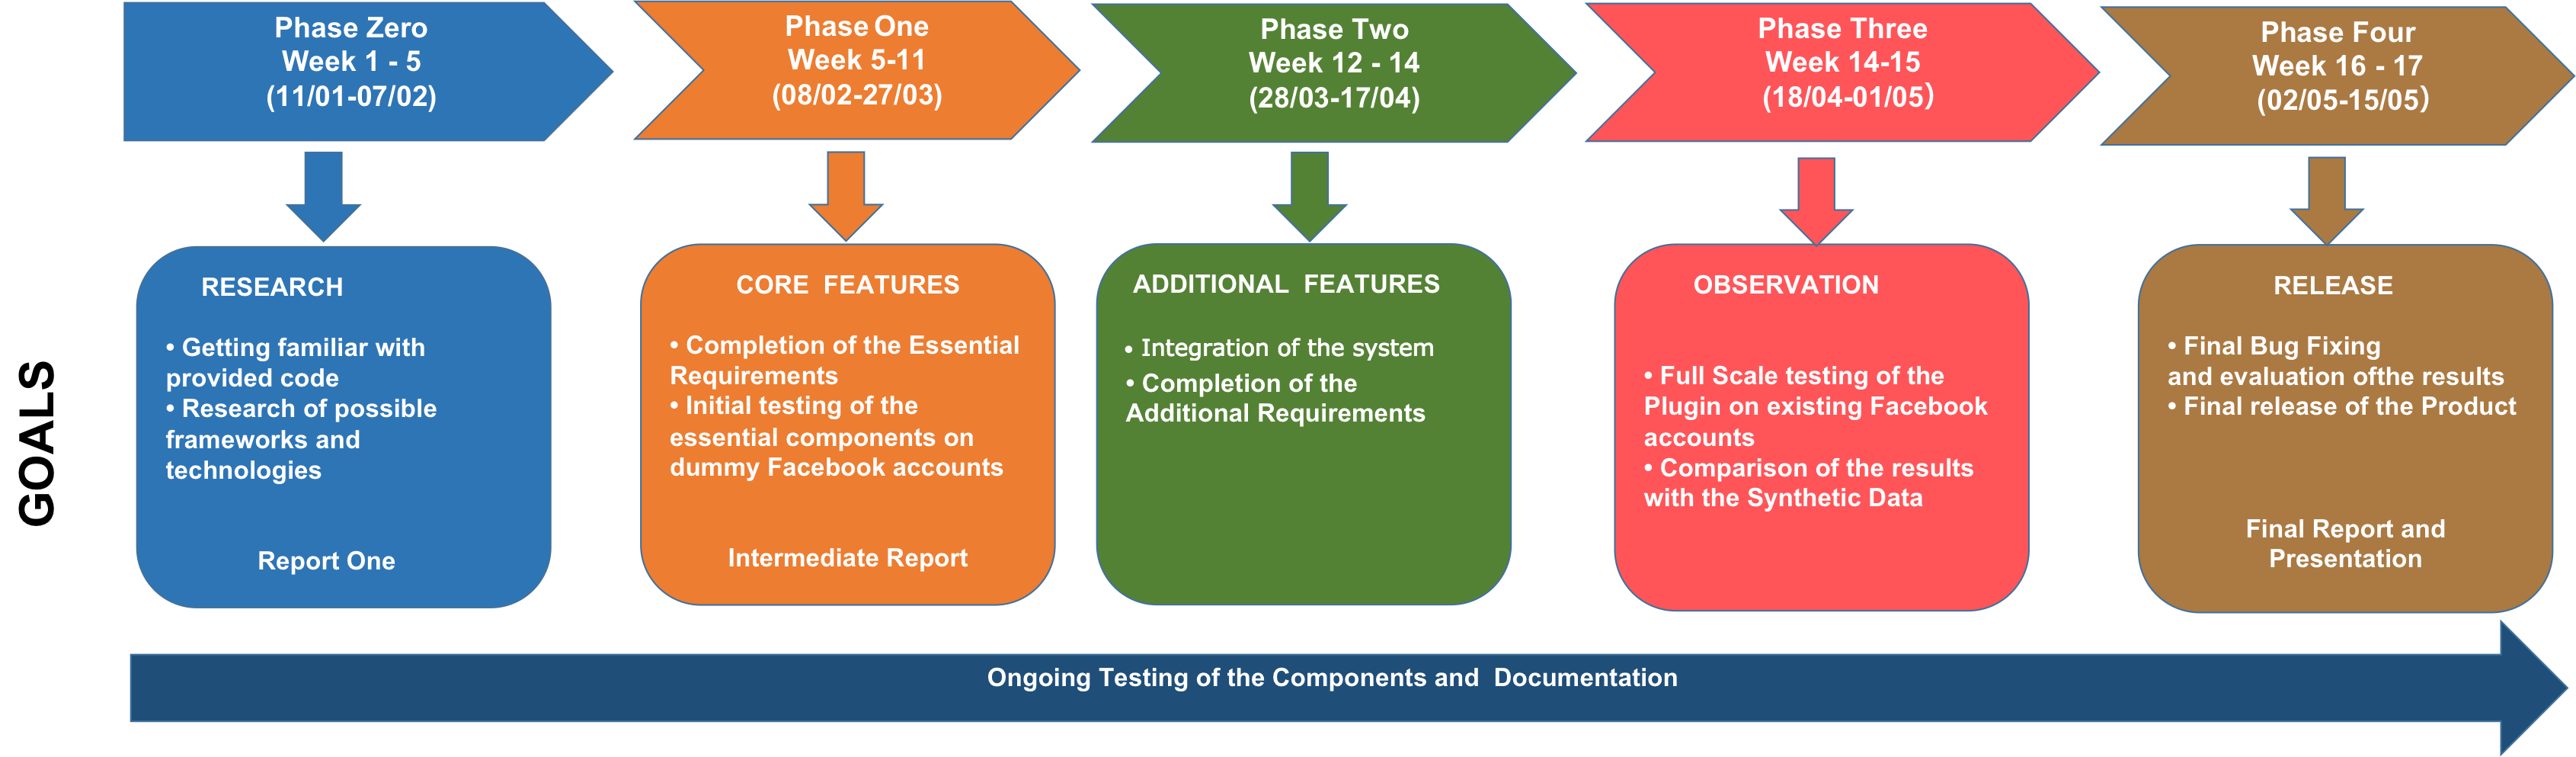
\includegraphics[scale=0.15]{Schedule}
	\caption{Updated Schedule}
\end{figure}

\subsubsection{Removed}

\begin{itemize}

\item \textbf{Adjusting the learning model to fit Facebook's new "reactions":} This task proved to be too challenging as the whole learning model had to be changed. Furthermore, there are many more states to account for and more factors to consider. For example, if someone expresses anger towards a user's post, it is not considered a privacy risk as no information is leaked, however, it is also not a social benefit as anger is not a positive emotion. 

\item \textbf{Obtaining permissions from Facebook to request the user for permissions to use their information:} Facebook has been extremely strict with regard to allowing use of their permissions. After repeated submissions, it was decided that obtaining permissions was not feasible.

\end{itemize}


\section{Design}

The proposed Learn to Share approach consists of two fundamental aspects, being social benefit and privacy risk of sharing information. Social benefits is represented by positive response gained through sharing of the information, whereas the privacy risk is defined as the risk of being exposed to sharing sensitive information with an improper audience.\\
\indent In order to evaluate the said privacy risk and social benefit, the research group proposes a web plugin that dynamically monitors interactions between the user and group members, categorising them into one of the predefined groups based on their potential privacy violation and displays an appropriate warning message, if necessary. 

\subsection{System Architecture}

\begin{figure}[H]
	\centering
	\includegraphics[scale=0.45]{ComponentDiagram}
	\caption{Component Diagram}
\end{figure}

Consequently, the most essential components that will make up the web plugin are as follows (Figure 1). 
\begin{itemize}

\item \textbf{Facebook API:}  The user logs in into Facebook and inputs the information along with the target audience. The API also allows the user to specify the social benefit and privacy risk thresholds, as well as the level of sensitivity. Besides, each piece of information, together with its corresponding level of sensitivity, is stored in the database.

\item \textbf{Parametric Model Checker:} Takes two essential parameters as inputs: a parametric Markov chain model and the user's sharing preference for the social benefit requirement, which can be obtained through probabilistic calculation tree logic (PCTL) formula. The latter one is an algebraic expression produced using an open-source probabilistic model checker, PRISM.

\item \textbf{Monitor:} Keeps track of the interactions on the user\textquotesingle s posts, which will be used in the learning model.

\item \textbf{Online Parameter Learning Engine:} Updates the model parameters

\item \textbf{Adaptive Sharing Analyzer:} Uses the updated parameters that are used to calculate the privacy risk and social benefit. The calculated values are then compared with the user- specified thresholds to estimate the trade-off, which is then used to determine if the information is safe to be shared with the selected audience.

\end{itemize}

\subsection{Program Flow}
\indent Furthermore, Figure 2 depicts more detailed sequence of activities of the web plugin. 

\begin{figure}[H]
	\centering
	\includegraphics[scale=0.45]{ActivityDiagram}
	\caption{Activity Diagram of the plugin}
\end{figure}

\subsection{Monitor Design} 

Monitor is the key component of the back-end and is responsible for keeping track of interaction between the user and friends. Monitor class should fetch the user’s friend list and follow-up all interaction a user may have during the plugin running time. Therefore, if somebody comments on a user’s post or presses the Like button or re-shares it, the Monitor should be able to fetch the information related to this interaction including the ID of that person or the date and time of the interaction. Accordingly, a set of tools is required to communicate with Facebook database and access related data. These tools have generally been provided by Facebook.

\subsubsection{Facebook Platform}

The Facebook Platform is a set of tools and services provided by Facebook for software developers to create applications accessing data in Facebook database. Using this platform, third-party developers are provided with a set of programming interfaces that enable them to interact Facebook features. 

\subsubsection{Graph API}
The Graph API is the backbone of Facebook Platform [Ref]. Technically, a social graph depicted personal relations within a social network. In this representation, nodes represent users and the friendship relationship is represented by edges.
\\
\indent Facebook Graph API is demonstrations of Facebook social graph so as objects, including people, pages, and events, and their connections, such as relationships and shared contents, are accessible by developers.  As the structured view of data, the Graph API is the primary way to get data in and out of Facebook’s platform.
\\
\indent Being a low-level HTTP-based API, working with the Facebook Graph API can be demanding. There are some libraries that can facilitate implementing this API. 

\subsubsection{Programming Languages and Libraries}

The existing base code for the Online Learning Model is initially in Java. Moreover, the lack of system dependency of the language and widely availability made Java a reasonable choice for back-end programming and led to less integration complexity. For employing Facebook Graph API,there are two prominent Java-based libraries: 

\begin{itemize}

\item \textbf{RestFB:} An open source Facebook Graph API client written in Java. It provides some simple but powerful operative programming tools to fetch information from or publish new information to Facebook.

\item \textbf{Facebook4J:} Another unofficial Java library for the Facebook Graph API. This library is also based on Java and provides some simple tools to integrate an application with the Facebook API.


\end{itemize}

For using these libraries, the related .jar file should only be added to the application class path. RestFB is more flexible and popular. There is also good documentation available for this library. Consequently, this library was chosen for this project.

\subsubsection{Access Token}
To have access to make graph API calls using the RestFB client, an access token is needed. An access token is a long string of characters that is an identification of the user and can be used by an app, in this case the plugin, to make graph API calls. Access tokens have different types and can be obtained via a number of methods. Within the scope of this project, UserAccess Token has been required. The user token is the most commonly used type of tokens that is required whenever an app calls an API to read or write a specific data on the user’s Facebook. This token can be obtained via a login dialog and getting the user’s permission so that enables the app to obtain the access token. It is also can be acquired manually through Graph API Explorer presented in the Facebook developers tools. 

\subsubsection{Implementation}

The most important consideration in establishing the Monitor class is that it should not miss any interaction. It means that after running the plugin, every social interaction between the user and a friend should be taken into account in the learning procedure. Consequently, the Monitor should be efficient in performance because, in a possible scenario, the user may want to upload next information, immediately after the last one. In this case, the Monitor should be able to track the interactions on the most recent post, as well.
\\
Furthermore, due to the research paper, in the learning to share approach, to evaluate each friend’s behavior, the parameters should be calculated for each friend separately. Thus, in each learning procedure, the Monitor should be run n times, where n is the number of the user’s friends. If this execution happens serially for a user who has many friends, it cannot be efficient enough to follow-up the recent interactions. Therefore, the Monitor should be developed in a multithreading manner in which a thread will be created per each friend and each of them is responsible to monitor interactions with that special friend.
\\
There are two main possible ways to implement the Monitor. The first naïve way is going through all the information that the user has alreadyposted and calculating the parameters due to the interactions. Although this scheme is easy to implement, it is not feasible for users who havemany posts; if there are a lot of posts and interactions per each of them, the learning procedure will be computationally expensive and most of the recent interactions may be missed.
\\
Another way is using Facebook notifications to keep track of the interactions. As it has already been explained, when an interaction happens, the user will get a notification. Thus, when the plugin starts to run, the Monitor should only listen to the notifications that the user gets. In this approach, at the beginning, it has been assumed that all the user’s friends are privacy-aware without any malicious behavior. Then, as the time proceeds, the interactions will be captured by parsing the incoming notifications and the parameters will be calculated, consequently. 

\subsection{Structure of the plugin}
The plugin consists of the following main elements:

\begin{itemize}

\item \textbf{Manifest:} a JSON-formatted file that includes the data and instructions about the plugin itself, such us the name, version and security settings.

\item \textbf{Popup.js:} a JavaScript file responsible for the manual interaction with the plugin through the pop up.

\item \textbf{Popup.html:} a file containing iframe to the web service.

\item \textbf{Contentscript.js:} a file responsible for creation of an iframe for warning messages.

\end{itemize}

It must be mentioned that in order to provide with as much encapsulation of information as possible, the plugin component that ought to be installed by the user was developed to consist of the iframe tag solely, as opposed to containing any program logic. With such a choice, the iframe tag points to a relevant page, being the login, terms and conditions, sensitivity settings and a warning message that is served by the plugin web service. Such an approach not only ensured that the code is encapsulated, but it also made the overall design of the project much easier, as the communication between the monitor and the plugin was therefore possible without implementing additional communication services. \\
\indent There were several other choices that were considered in this project as opposed to the usage of iframes. Here write it up if I manage to fix the issue  

\subsection{Structure of Web Service}

The web service consists of the following elements:

\begin{itemize}

\item the backend server

\item the frontend components

\item database

\end{itemize}

Here flowchart 

The backend server serves the frontend components in the order depicted by the Figure X. User information such as user id, set sensitivity level an message id (obtained from the monitor component) and user were then stored in the database to be reused accordingly.

\subsection{Web Service Implementation}

\subsubsection{Backend}

\textbf{Web Service Host}\\
The web service is hosted using AWS (Amazon Web Service) cloud computing platform . AWS delivers high availability performance, including bringing servers online and offline very quickly, and offering storage system that is capable of vast scaling. Moreover, AWS is very flexible, as all the services work and communicate together with your application to automatically judge demand and handle it accordingly . Other platforms considered for this project were Digital Ocean and Microsoft Azure, however AWS appealed as the most user-friendly, secure and flexible platform to all team members.\\\\

\noindent \textbf{MVC Framework}
\\
As far as the Web Service is concerned, the MVC frameworks that were considered for this project included GWT (Google Web Toolkit), Spring and Spring Boot – a “simplified” MVC framework based on Spring. As this web service is the first web application attempted by all team members, it was important to select a framework that would be simple to learn and easy to use.
\\
\indent Although GTW seemed to be an easy to learn, well documented framework, according to research conducted by RebelLabs , out of 2164 JVM developers, over 70\% stated that other frameworks must be used in addition to GTW to ensure the most optimal implementation of the service. That was not ideal for this project, as this would introduce additional complexity, risking the delivery of the final product within deadline.
\\
\indent Spring framework, on the other hand, was considered due to its popularity, reliability and flexibility related to settings available to support the project. However, such flexibility appeared to bring a huge disadvantage – it proved difficult and time consuming to set up the project as such. As a result, more research was conducted to find something as reliable and flexible as Spring, yet less difficult to configure and maintain. Spring Boot, therefore, became an obvious choice for this project, as it provides the shortest way to have a Spring web and it is a pre-configured, pre-sugared set of frameworks/technologies to reduce that boiler plate configuration.
\\\\
\textbf{Database}
\\
It was concluded after extensive research that MongoDB would be a perfect choice for this particular project. The main reason why such choice was made is the fact that it is easy to use and maintain and comes pre-set with Spring Boot. MongoDB is an open source NoSQL database that uses a document-oriented data model. Like other NoSQL databases, MongoDB uses dynamic schema, allowing the documents in a collection to have different fields and structures. The database stores data in JSON-like documents that can vary in structure. Related information is stored together for fast query access through the MongoDB query language.That made MongoDB a perfect choice for this particular project, as a majority of group members did not have any previous experience with SQL, therefore querying in Java was the best and fastest option. 

\subsection{Front End}

\subsubsection{The Design Process}

The idea behind the overall design was to provide the user with sense of security by using calming colour pallet of blues with the mixture of purple. The design as such was also supposed to subtly remind the user of Facebook, ensuring at the same time that the plugin does not entirely look like a Facebook’s product, which could have had potential legal implications.
\\\\
\textbf{Logo Development}\\
The project required two logo designs – one to be used as an icon displayed in the browser’s toolbar, and the second to be featured as a plugin’s header. The icon’s design had to be as clear as possible due to low visibility of the icon, whereas the header was required to provide the user with more information on the product.
\\
\indent The initial idea behind the icon was to create a shield-like shape to emphasise on the protection provided by the plugin, as well as containing “Learn To Share” initials and a red BETA flag. However, after using the icon on a tester plugin, it was observed that the LTS initials were completely unreadable. This discovery led to further research1 that inspired more minimalistic design that was not only visible, but also sent a clearer message of the plugin as a security tool for Facebook. The Beta flag and name of the product had to be discarded, as these were not visible at all in the Chrome toolbar.
\\
As the header logo did not have visibility constraints, it was decided that the BETA flag and the product name should be displayed here instead. Thecolours were also changed to white, as the dark blue background provided with a contrast to the overall design of other web pages, drawing user’s attention to the header in an instant. 
\\
\textbf{Design of pages and warning message}\\
The design of pages as such was aimed to remind the user of Facebook,therefore a similar white and grey colour pallet was applied. Moreover, as the plugin is a small-sized product, the best option was to apply a minimalistic design.
\\
The design aim with regard to warning message, on the other hand, was to ensure it could stand out on user’s Facebook page, without being too intrusive. Two designs were considered in particular: one featuring an exclamation mark in a shield, along with the message with Learn To Share header. It was concluded that the design with an exclamation mark would be too
\\
Initially, the plugin was also meant to include the loading wheel to indicate to the user that the request is currently being processed. However, without AJAX one page web service, the loading wheel would cause the header to re-load frequently, providing with unpleasant user experience. Although discarded, the design can still be viewed in the Appedix Z.
\\

\subsection{Implementation and Design}

Each page was designed to be implemented as a separate static web page. The structure of the front end was also considered to be developed as a one-page web service loaded using AJAX injections. That would allow the header to never require re-loading, allowing for better user experience. This alternative design would consist of a main page template, being a header and an empty container, as well as separate small page elements that would be loaded into the container accordingly. Although sounding very appealing, the idea was discarded as too risky to implement. The reasoning behind such was the fact that the plugin element was built on the basis of iframes, therefore introducing multiple iframe-like technologies could also introduce unnecessary bugs and could be hard to maintain and debug as such.

\subsubsection{CSS Frameworks and Libraries}
The purpose of the front-end CSS frameworks is to ensure the consistency across internal tools by providing with templates for HTML and CSS-based designs and optional JS extensions to animate certain web components. Before frameworks, various libraries were used for each component of the interface development separately, meaning inconsistencies and high maintenance1. Although the design required for the plugin was not extensive, it was concluded that in this case the implementation of a framework was the most optimal choice that would provide with the most professional look in the shortest amount of time. That would not be possible to achieve by first-time programmers by writing own CSS framework. After exploring several options, including Bootstrap, Semantic UI, Pure and Kube CSS, it was concluded that an open source Kube CSS would be the best choice for this project, as it provides with simple to use and beautiful to look at designs. Although not as popular as Bootstrap that has been favoured over 90,000 times on Github2, nor was developed by a well-known company, Kube CSS’s minimalistic designs appear perfect for a small project like a plugin. 
\\
\indent Additionally, jQuery’s Slider3 along with Lugo Lab’s Flat Slider4 libraries were used to achieve a perfect look for the Sensitivity Level slider.

\subsubsection{JavaScript Frameworks}
As the project included only a small section of JavaScript that was used for only for the sensitivity setting and AJAX requests, the use of a client-side JavaScript framework as such was not of a necessity. Although the CSS and HTML content for the plugin was also not extensive, the use of framework was most optimal choice in that instance, as CSS frameworks provide with.
\\
\indent Although frameworks like EmberJS or React are thought of as industry-standard practice, the setting time of the framework for such a small section would not be practical and therefore this part of the project was developed using vanilla JavaScript.

\section {Methodology}

\subsection{Development Technique}
Due to schedule constraints and lack of previous software development experience, the development process will take place iteratively\cite{SoftwareEngineering}. Such approach allows for creation of mini-projects, which appears to be less risky than a spiral model in the instance where additional features would not be possible to implement. 
\\ 
\indent Moreover, the project adopted the Agile ideology\cite{Scrum} with Scrum framework. The reasoning behind such is more flexible model of Scrum over XP, and a greater suitability for smaller, as in this instance, development teams. Also, Scrum will enable a more efficient development of the plugin by more structured process through division of work into tickets. To ensure the group maintains the agile development structure throughout the process, the use of Trello\cite{trello} software for the ticketing purposes, and Asana\cite{asana} for the project management was used.
\\
\indent A backlog was created on Trello in order to keep track of what needs to be done and a board for each phase to allow each member to update the status of their task as well as stay updated on each others progress.

\subsection{Version Control}
As far as the version control system is concerned, the distributed approach as opposed to centralized was adopted due to the flexibility it offers and the option to work on several features simultaneously\cite{Design}. Although it is believed that distributed model could be more difficult to maintain and prone to merge conflicts\cite{Design}, previous experience with the Git-based software, along with daily meetings reduced such risks to minimum. Moreover, GitHub was decided upon over Mercurial and other distributed VCSs, due to reliability, popularity and an excellent logging capability\cite{GitHub}.

\subsection{Implementation}

\subsubsection{Monitor}

The monitor was written in Java and utilises the RestFB client which provided methods to make calls to the Facebook Graph API to retrieve the data required. The methods were sufficient for the program to work. However, the access token for the corresponding user needs to be provided in order for the methods to work and this has to be retrieved by some other way.
\\
\indent Some users may have a large number of friends and posts, so retrieving data and processing it for all of these friends may be computationally expensive and slow. Concurrency was introduced into the program, so that one instance of the monitor runs for each friend concurrently. Furthermore, only the most recent posts were taken into account, so that the program does not have to look through so many posts. 
\\
\indent For each post, the monitor identifies the interactions that the friend has made on the post as well as the level of sensitivity of the post and passes this information to the next component to perform the calculations for the learnt probabilities.

\subsubsection{Adaptive Sharing Analyzer}

The adaptive sharing analyzer takes in the learnt probabilities 

\subsection{Facebook Limitations}
\begin{enumerate}
\item The user's notifications are required in the monitor to keep track of the interactions on the user's posts. However, the latest version (2.5) of the Facebook graph application programming interface (API)\cite{GraphAPI} does not allow access to the \textbf{manage\_notifications} permission. Hence, a lower version (2.2) has to be used.

\item Only the Facebook notifications that have not been read by the user are obtainable through the API. Therefore, the program might miss some of the interactions if the user has already read them. A possible solution for this issue is employing Facebook webhooks which allows the plugin to become aware of new notifications.

\item Another problem with the notifications can happen when multiple instances of the same interaction occur on the same post by multiple friends; Facebook groups these interactions under the same notification ID which only provides the ID of the friend who interacted most recently. To solve this problem, the names of the friends who interacted were retrieved by parsing the notification messages. 

\item Facebook recently introduced a new feature called reactions\cite{FBreactions}. Other emotions can now be expressed for a post in addition to liking it. These reactions are "Love", "Haha", "Wow", "Sad" and "Angry". Thus, the learning model has to be readjusted to fit these.

\item To create a plugin where the user can login to Facebook and give the plugin the required permissions, a proposal along with screenshots must be submitted to Facebook explaining how the permissions will be used, To do this, a prototype of the plugin that demonstrates the use of these permissions safely must first be created. 
\end{enumerate}

\subsection {Plugin Component Issues}
\begin{enumerate}
\item The current design of the plugin component as illustrated in Appendix A consists of two elements - the settings section and the warning message section\cite{AppType}. The settings section element is only visible once user manually presses the browser’s plugin button – using the “popup” approach. The second section is automatically triggered on mouse hover over a specific page element, therefore having knowledge of Facebook\textquotesingle s DOM (Document Object Model). It was not known at the time that these two were considered as different types of extensions, and that both need to be synchronized with a complex messaging system\cite{MessagePassing}. The delay caused by the synchronisation could have been avoided if more thorough research took place initially. 

\item The dynamic structure of Facebook\textquotesingle s page poses a significant threat to reliability of the plugin development using the DOM-oriented approach, as it may prove impossible to target specific HTML tags for the triggering event due to ever-changing names of the elements. Additionally, it is possible that Facebook may not approve of manipulation of its DOM at all, which is currently being enquired about at Facebook. Therefore, there is a high possibility that splitting the plugin into two elements can be marked as a high-risk element or no longer feasible. An alternative solution may include moving the entire warning system to the sensitivity input section, providing with notification system that does not interfere with the Facebook\textquotesingle s DOM.

\item After reading the Facebook Platform Policy\cite{FBpolicy}, it was discovered that it is necessary to obtain user\textquotesingle s consent prior to user\textquotesingle s login to use Facebook API. Therefore the new requirement, being terms and conditions screen was added.
\end{enumerate}



\subsection {Testing Methodology}

\subsubsection {Unit testing}
For the monitor component, the RestFB 1.19 API\cite{RestFB} for Java is used to make calls to Facebook's API to retrieve data.  Therefore, a Black-Box approach was taken in order to test the methods provided by RestFB. Dummy Facebook accounts have been created and manual tests were written in JUnit\cite{JUnit} in order to check that each function defined by RestFB is able to provide the required data from the dummy accounts for the plugin. The testing process provided an understanding of the functionality of the API as well as its limitations, which was helpful in determining the best way to implement the methods.
\\
\indent For each of the other Java classes, a White-Box approach was taken. Synthetic data was used for each of the methods and the output was tested against the expected results. Each test case was written in JUnit and the synthetic data was generated to cover all branches in order to maximize code coverage. For example, the Adaptive Sharing Analyser takes in an array of learnt transition probabilities and the sensitivity level for a piece of information as inputs and returns one of three values (0.0 means do not share; 0.5 means give a warning message; 1.0 means safe to share). The transition probabilities were generated to simulate the different types of behaviours and each array of probabilities was tested with different levels of sensitivity and compared with the expected output. All the tests were put together into a test suite which checks the overall testing results. The JUnit test results can be found in Appendix B.
\\
\indent EclEmma\cite{EclEmma}, an Eclipse code coverage tool, was used to generate the code coverage report for each of the tests. The table below shows the code coverage of the tests.

 \begin{table}[H]
\centering
\captionof{table}{Code Coverage for Java classes} \label{tab:title2}
 \begin{tabular}{|c|c c|}
 \hline
 Class & Instruction Coverage & Branch Coverage\\

\hline
Monitor & 98.9 \% & 100.0\%\\
Transition Probability & 92.5\% & 100.0\%\\
Adaptive Sharing Analyser & 94.3\%& 75.0\%\\
Social Benefit Calculator &99.6\%& 83.3\%\\
Privacy Risk Calculator &100.0\%& 100.0\%\\
\hline
Overall Coverage &94.2\%&87.0\%\\
\hline
 \end{tabular}
 \end{table}

The vanilla JavaScript and JQuery unit tests will be completed using QUnit\cite{QUnit} once the integration of the plugin takes place, as the majority of the code communicates with Facebook and the server.

\subsubsection {Accuracy Testing}
As part of system testing, emphasis was placed on sensitivity and specificity\cite{SnS}. The results from the tests helped to determine the best parameter values for the plugin to have an accurate determination of the respective friends' behaviours.
\\
\indent To do this, a test was be run for each parameter value used in the learning model. For each experiment, simulating either an immediate harmful behaviour pattern or delayed harmful behaviour pattern, and varying either the privacy risk threshold ($W_i^{PR}$) or the social benefit threshold ($W_i^{SB}$). Each experiment was run ten times and the average values were used.
\\
\indent Synthetically generated data was used to model different behaviours. For each behaviour, the test involved varying the parameter intended for testing and recording the number of true positive(TP), false positive(FP), true negative(TN) and false negative(FN) suggestions made by the system.  Each kind of output is specified as follows:
\begin{itemize}
\item TP: the number of times the system guided the user to share the item of information with friend j, and j's actual re-share probability was within the acceptable range; the times the system guided the user not to share and both system requirements were violated;

\item FP: the number of times the system flagged a warning and one of the two system requirements($W_i^{PR}$ or $W_i^{SB}$) had been violated;

\item TN: the number of times the system guided the user not to share and only one of the system requirements was violated; the times the system guided the user to share the information with friend j, and j's actual re-share probability was above the acceptable range;

\item FN: the number of times the system flagged a warning and both system requirements had been violated;
\end{itemize}
Based on the results from the above experiment, the following will be used to measure the system performance.
\\Accuracy(ACC) measures how accurately it determines the sharing behaviour
\begin{align}
 &ACC: \frac{(\sum{TP} + \sum{TN})}{(\sum{FP} + \sum{FN} + \sum{TP} + \sum{TN})}
\end{align}
Sensitivity(TPR) measures the proportion of correctly identified positives
\begin{align}
 &TPR: \frac{\sum{TP}}{(\sum{TP} + \sum{FN})}
\end{align}
Specificity(SPC) meaning the proportion of correctly identified negatives formula 
\begin{align}
&SPC: \frac{\sum{TN}}{(\sum{FP} + \sum{TN})}
\end{align}

 \noindent In each computing result, the higher the value, the more efficiently it learned.

\section{Group Work}

The project was divided into four parts: The Monitor, User Interface and Server Implementation, Obtaining Facebook Permissions and Testing Framework. Each member was assigned to one part as seen in the table below.

 \begin{table}[H]
\centering
\captionof{table}{Division of Work} \label{tab:title2}
\hspace*{-0.3in}
 \begin{tabular}{|c|M{4cm}|M{4cm}|c|}
 \hline
\textbf{Monitor} & \textbf{User Interface and Server} & \textbf{Obtaining Facebook Persmissions} & \textbf{Testing Framework}\\

\hline
Boon Eng Oh & Magdalena Sadowska & Shanshan Fu & Yunxin Zhou \\


Shahi Shahrokh & & & Ani Petrosyan \\
\hline
 \end{tabular}
 \end{table}

For the monitor, Boon worked on integration of the monitor with the other parts of the plugin while Shahrokh worked on fetching the required data using the RestFB API.\\
\indent 

\section{Final Product}

Unfortunately, due to Facebook's strict regulations, the permissions required to request the user for the required permissions through a user interface could not be obtained. 

The final product is able to identify some behaviour patterns correctly and peform the appropriate action for these friends. 


\bibliographystyle{plain}
\begin{thebibliography}{9}
\bibitem{InternetUsers}
eMarketer. 2014. 
\emph{Internet to Hit 3 Billion Users in 2015.} [ONLINE]. Available at
\url{http://www.emarketer.com/Article/Internet-Hit-3-Billion-Users-2015/1011602}[Accessed 23 January 16]
\bibitem{PrivacyBreaches}
	Xu, H., Teo, H.H., Tan, B.C. and Agarwal, R., 2009.
	The role of push-pull technology in privacy calculus: the case of location-based services.
	\emph{Journal of Management Information Systems},
	26(3), pp.135-174. 
\bibitem{FacebookRegret}
	Wang, Y., Leon, P.G., Chen, X. and Komanduri, S., 2013. From Facebook regrets to facebook privacy nudges.
	\emph{Ohio St. LJ, 74}, p.1307.
\bibitem{ShareRegret}
	Wang, Y., Norcie, G., Komanduri, S., Acquisti, A., Leon, P.G. and Cranor, L.F., 2011, July. I regretted the minute I pressed share: A qualitative study of regrets on Facebook. 
	\emph{In Proceedings of the Seventh Symposium on Usable Privacy and Security} (p. 10). ACM.
\bibitem{RankSN}
	Statista. 2016. 
	\emph{Leading social networks worldwide as of January 2016, ranked by number of active users (in millions).}[ONLINE]. 				Available at \url{http://www.statista.com/statistics/272014/global-social-networks-ranked-by-number-of-users/}[Accessed 26
	January 16].
\bibitem{Interactions}
	Yang, M., Yu, Y., Bandara, A.K. and Nuseibeh, B., 2014, September. 
	Adaptive sharing for online social networks: a trade-off between privacy risk and social benefit.
	\emph{In Trust, Security and Privacy in Computing and Communications (TrustCom), 2014 IEEE 13th International Conference on}(pp. 45-52). IEEE.
\bibitem{KAOS}
	Van Lamsweerde, A. and Letier, E., 2004. From object orientation to goal orientation: A paradigm shift for requirements engineering. In \emph{Radical Innovations of Software and Systems Engineering in the Future} (pp. 325-340). Springer Berlin Heidelberg.
\bibitem{Java}
	 Oracle.
	\emph{The Java Language Environment.}[ONLINE] Available at: 			\url{http://www.oracle.com/technetwork/java/intro-141743.html\#318} [Accessed 27 January 16].
\bibitem{SoftwareEngineering}
	Chang, S.K., 2002. 
	\emph{Handbook of Software Engineering \& Knowledge Engineering: Fundamentals.} (Vol. 1). World Scientific. 
\bibitem{Scrum}
	Sutherland, J., Schwaber, K., Scrum, C.C.O. and Sutherl, C.J., 2007. 
	\emph{The scrum papers: Nuts, bolts, and origins of an agile process.} 
\bibitem{trello}
	Trello.[ONLINE] Available at: \url{https://trello.com/}. [Accessed 01 February 16].
\bibitem{asana}
	Asana.[ONLINE] Available at: \url{https://app.asana.com/}. [Accessed 28 January 16].
\bibitem{Design}
	Hardeep, S., 2013, 
	\emph{Designing, Engineering, and Analyzing Reliable and Efficient Software.}
\bibitem{GitLab}
	Van Baarsen, J. 2014.
	\emph{GitLab Cookbook.} Packt Publishing Ltd.
\bibitem{GraphAPI}
	Facebook for developers. 2010. Facebook Graph API. [ONLINE] Available at: \url{https://developers.facebook.com/docs/graph-api}. [Accessed 06 March 16]. 
\bibitem{FBreactions}
	Facebook. 2006. Newsroom. [ONLINE] Available at: \url{http://newsroom.fb.com/news/2016/02/reactions-now-available-globally/}. [Accessed 06 March 16].
\bibitem{AppType}
	Google Chrome. Choosing an App Type. [ONLINE] Available at: \url{https://developer.chrome.com/webstore/choosing}. [Accessed 05 March 16].
\bibitem{MessagePassing}
	Google Chrome. Message Passing. [ONLINE] Available at: \url{https://developer.chrome.com/extensions/messaging}. [Accessed 06 March 16].
\bibitem{FBpolicy}
	Facebook for developers. Platform Policy. [ONLINE] Available at: \url{https://developers.facebook.com/policy/}. [Accessed 01 March 16].
\bibitem{RestFB}
	RestFB 1.20.0. 2010. Overview. [ONLINE] Available at: \url{http://restfb.com/javadoc/}. [Accessed 05 March 16].
\bibitem{JUnit}
	Tahchiev, P., Leme, F., Massol, V. and Gregory, G., 2010. JUnit in action. Manning Publications Co..
\bibitem{EclEmma}
	EclEmma. 2006. Java Code Coverage for Eclipse . [ONLINE] Available at: \url{http://eclemma.org/userdoc/}. [Accessed 03 March 16].
\bibitem{QUnit}
	Sheiko, D., 2013. Instant Testing with QUnit. Packt Publishing Ltd.
\bibitem{SnS}
	Flach, P., 2012. Machine learning: the art and science of algorithms that make sense of data. Cambridge University Press. 
\end{thebibliography}

\newpage
\appendix

\setcounter{figure}{0} 
\captionsetup{skip=3pt}
\section{User Plugin Mockups}

\vspace{1mm}
\begin{figure}[H]
	\centering
	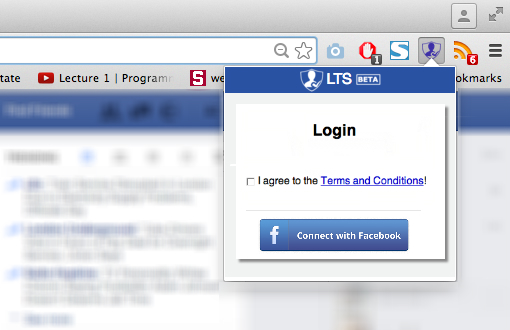
\includegraphics[scale=0.52]{APpendix/LoginScreen}
	\caption{Login Screen}
\end{figure}

\begin{figure}[H]
	\centering
	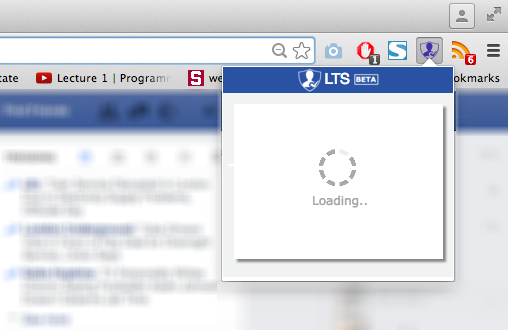
\includegraphics[scale=0.52]{APpendix/LoadingScreen}
	\caption{Loading Screen}
\end{figure}

\begin{figure}[H]
	\centering
	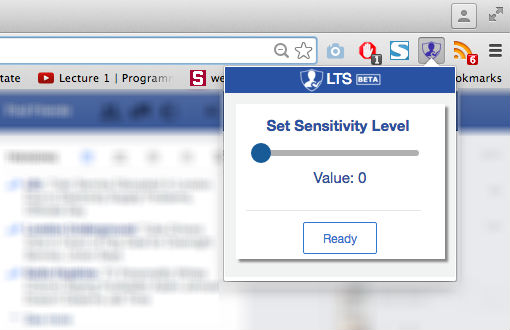
\includegraphics[scale=0.52]{APpendix/SenInput}
	\caption{Sensitivity Input}
\end{figure}

\begin{figure}[H]
	\centering
	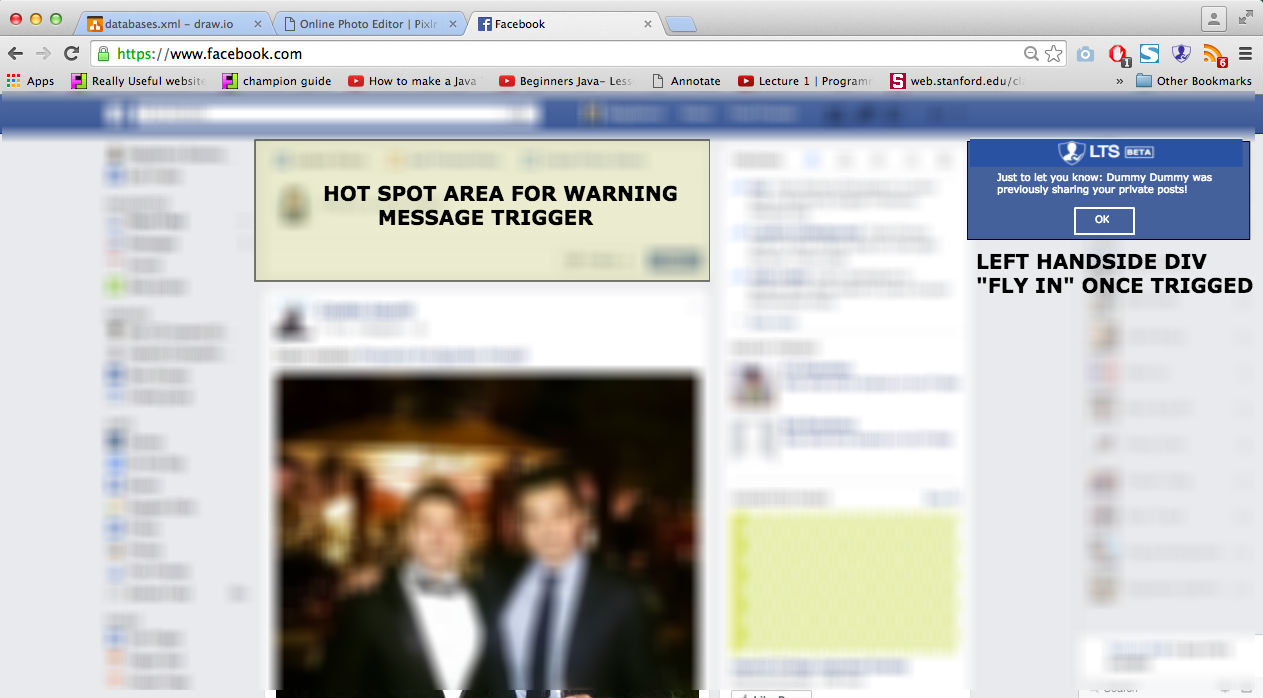
\includegraphics[scale=0.32]{APpendix/WarnMessage}
	\caption{Warning message}
\end{figure}
\vspace{1cm}
\begin{figure}[H]
	\centering
	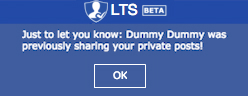
\includegraphics[scale=0.72]{APpendix/warnpopup}
	\caption{Warning Popup}
\end{figure}
\vspace{1cm}

\begin{figure}[H]
	\centering
	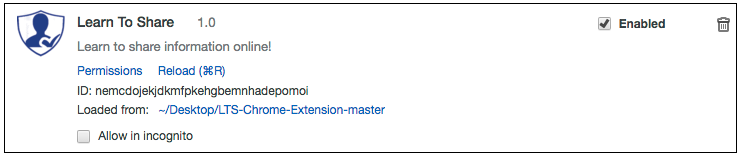
\includegraphics[scale=0.725]{APpendix/lts2}
	\caption{Chrome Extension}
\end{figure}

\section{Test Results}

\begin{figure}[H]
\centering
\vspace{1cm}
\begin{subfigure}{.5\textwidth}
  \centering
  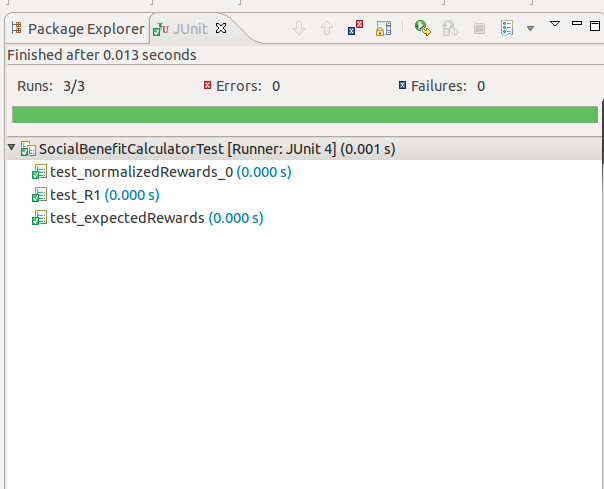
\includegraphics[scale=0.42]{APpendix/SBTest}
  \caption{Social Benefit Calculator Test}
\end{subfigure}%
\begin{subfigure}{.5\textwidth}
  \centering
  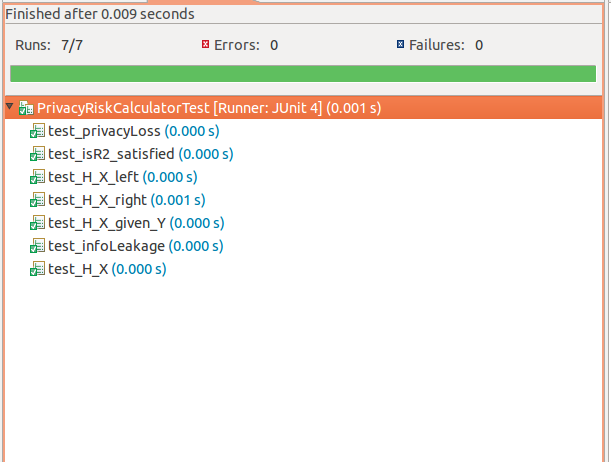
\includegraphics[scale=0.42]{APpendix/PRTest}
  \caption{Privacy Risk Calculator Test}
  \label{fig:sub2}
\end{subfigure}
\vspace{1cm}
\begin{subfigure}{.5\textwidth}
  \centering
  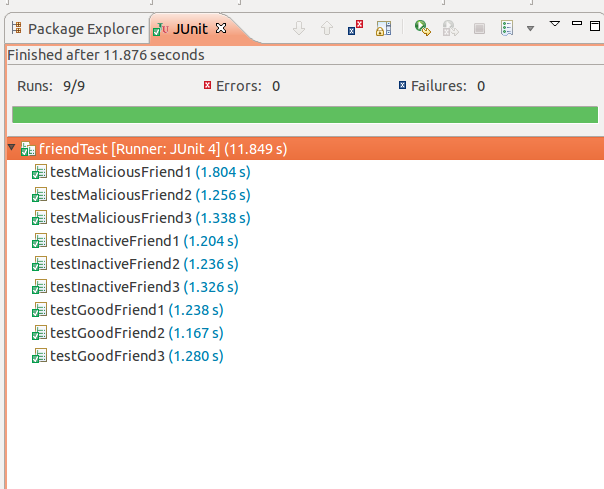
\includegraphics[scale=0.42]{APpendix/ASATest}
  \caption{Adaptive Sharing Analyser Test}
  \label{fig:sub1}
\end{subfigure}%
\begin{subfigure}{.5\textwidth}
  \centering
  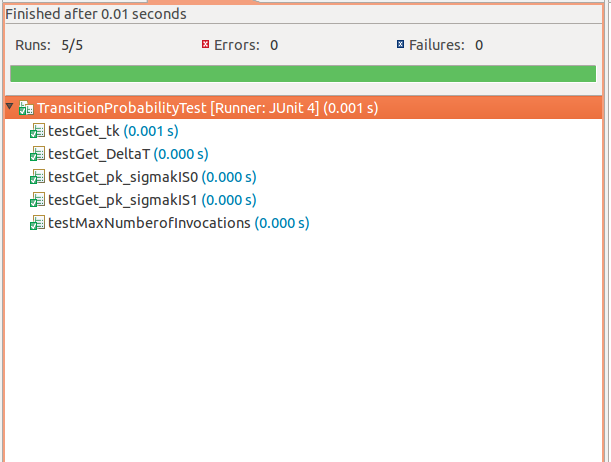
\includegraphics[scale=0.42]{APpendix/TPTest}
  \caption{Transition Probability Test}
  \label{fig:sub2}
\end{subfigure}
\vspace{1cm}
\begin{subfigure}{.5\textwidth}
  \centering
  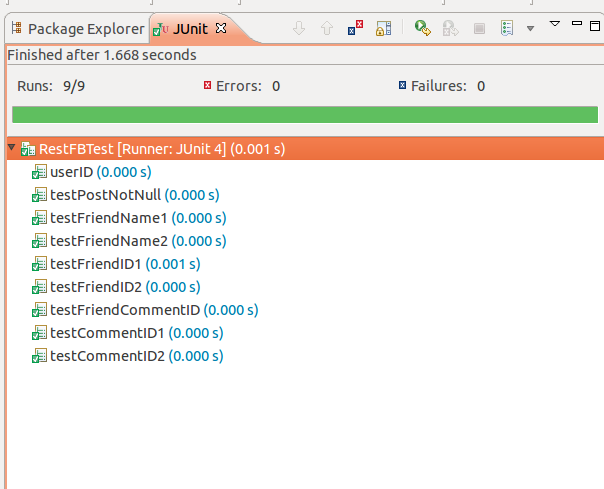
\includegraphics[scale=0.42]{APpendix/RestFBTest}
  \caption{RestFB Test}
  \label{fig:sub1}
\end{subfigure}
\end{figure}

\newpage
\begin{figure}[H]
	\hspace*{-0.0in}
	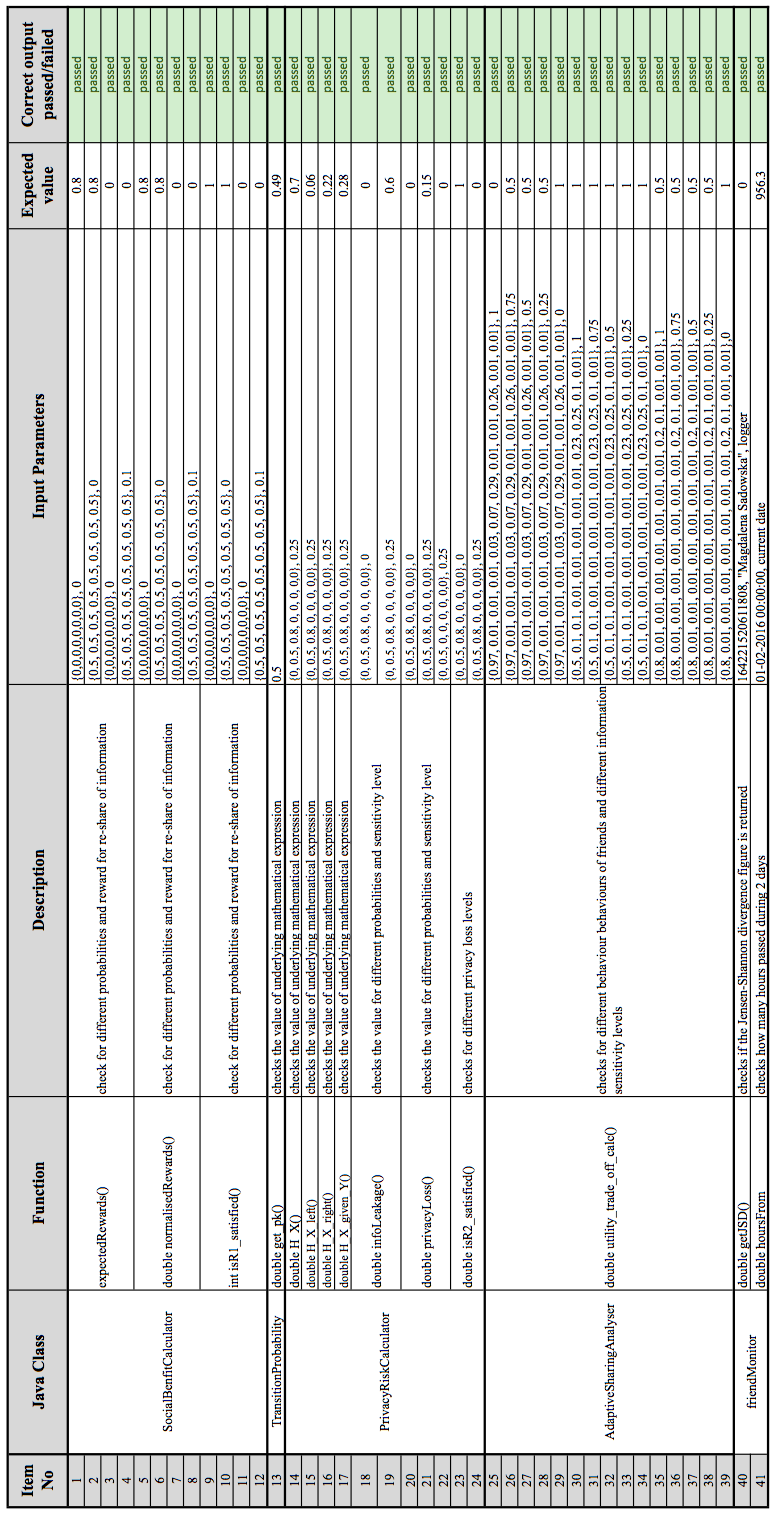
\includegraphics[width=1.0\textwidth,height=1.5\textwidth]{APpendix/tableResults2}
	\caption{JUnit Results}
\end{figure}

\section{Code Coverage Report}
\setcounter{figure}{0} 
\begin{figure}[H]
	\centering
	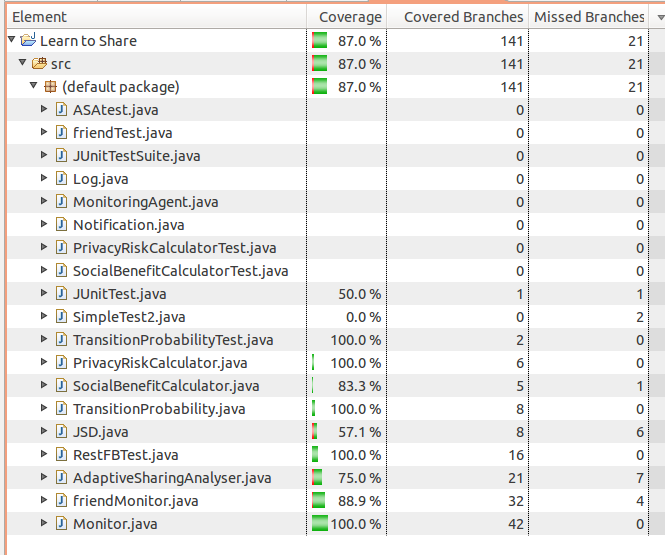
\includegraphics[scale=0.653]{APpendix/BranchCoverage}
	\caption{Branch Coverage}
\end{figure}


\begin{figure}[H]
	\centering
	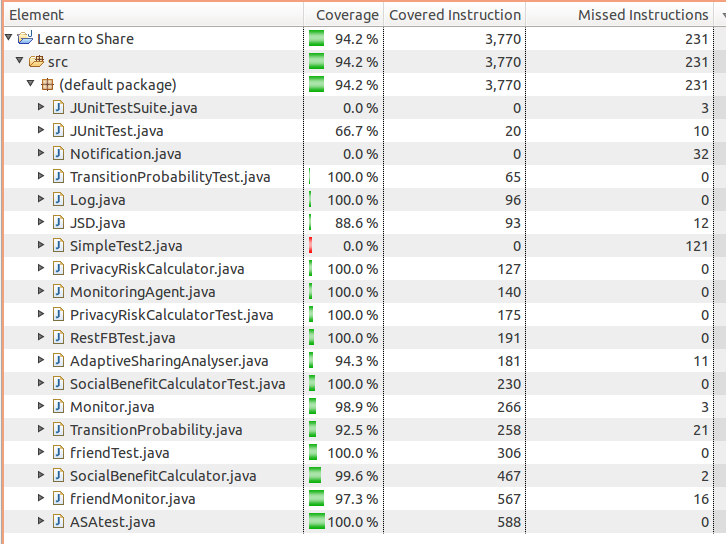
\includegraphics[scale=0.60]{APpendix/InstructionCoverage}
	\caption{Instruction Coverage}
\end{figure}


\begin{figure}[H]
	\centering
	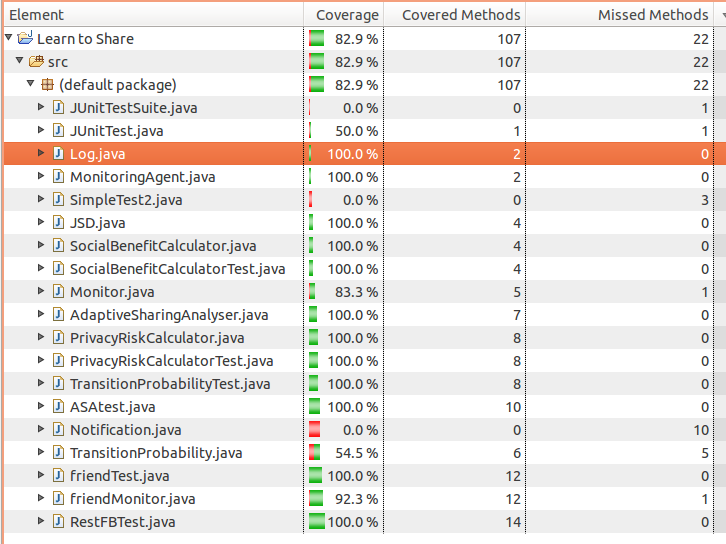
\includegraphics[scale=0.62]{APpendix/MethodCoverage}
	\caption{Method Coverage}
\end{figure}

\section{Logbook}




\end{document}

